\subsection{Undamped Forced Vibrations ($b = 0$)}
\noindent
Our equation now becomes
\begin{equation*}
	my'' + ky = F_0\cos{(\gamma t)}
\end{equation*}
We can use the method of undetermined coefficients to solve this system.\\

\noindent
Extracting the coefficients for the auxiliary equation and finding the roots,
\begin{equation*}
	mr^2 + k = 0 \implies r = \pm i\sqrt{\frac{k}{m}} = i\omega.
\end{equation*}
So, our homogeneous solution is
\begin{equation*}
	y_h = C_1\cos{(\omega t)} + C_2\sin{(\omega t)}.
\end{equation*}

\noindent
For guessing the form of $y_p$, we'll need to break into two cases depending on if $\omega = \gamma$. One case will give rise to beats and the other resonance.

\subsubsection{Beats ($\omega \neq \gamma$)}
\noindent
If $\omega \neq \gamma$, then we can guess that $y_p$ has the form
\begin{equation*}
	y_p = A\cos{(\gamma t)} + B\sin{(\gamma t)}.
\end{equation*}
Since we don't have a term involving the 1st derivative, we can be sure that $B = 0$, since an odd number of derivatives is the only way to turn a $\sin$ term into a $\cos$ term.
So,
\begin{equation*}
	y_p = A\cos{(\gamma t)}.
\end{equation*}
Solving for $A$,
\begin{align*}
	m\left(A\cos{(\gamma t)}\right)'' + k\left(A\cos{(\gamma t)}\right) &= F_0\cos{(\gamma t)} \\
	-mA\gamma^2\cos{(\gamma t)} + kA\cos{(\gamma t)} &= F_0\cos{(\gamma t)} \\
	A\left(k - m\gamma^2\right) &= F_0 \\
	A &= \frac{F_0}{k - m\gamma^2} = \frac{F_0}{m(\omega^2 - \gamma^2)}.
\end{align*}
So, our solution is
\begin{equation*}
	y = \frac{F_0}{m(\omega^2 - \gamma^2)}\cos{(\gamma t)} + C_1\cos{(\omega t)} + C_2\sin{(\omega t)}.
\end{equation*}\\

\noindent
Let's look specifically at the IVP where $y(0) = 0$ and $y'(0) = 0$.
\begin{equation*}
	C_1 = \frac{-F_0}{m(\omega^2 - \gamma^2)} \text{ and } C_2 = 0.
\end{equation*}
So,
\begin{equation*}
	y = \frac{F_0}{m(\omega^2 - \gamma^2)}\cos{(\gamma t)} - \frac{F_0}{m(\omega^2 - \gamma^2)}\cos{(\omega t)}.
\end{equation*}
Using the fact that $\cos{\alpha}-\cos{\beta} = 2\sin{\left(\frac{\alpha - \beta}{2}\right)}\sin{\left(\frac{\alpha + \beta}{2}\right)}$,
\begin{equation*}
	y = \frac{2F_0}{m(\omega^2 - \gamma^2)}\sin{\left(\frac{\gamma - \omega}{2}t\right)}\sin{\left(\frac{\gamma + \omega}{2}t\right)}.
\end{equation*}

\noindent
When $\gamma \approx \omega$, the $\gamma + \omega$, with a small period, dominates the motion, and the amplitude is slowly guided by the $\gamma - \omega$ term which has a large period.
This creates intervals guided by the $\gamma - \omega$ term of higher and lower amplitudes.
These are beats.

\begin{center}
	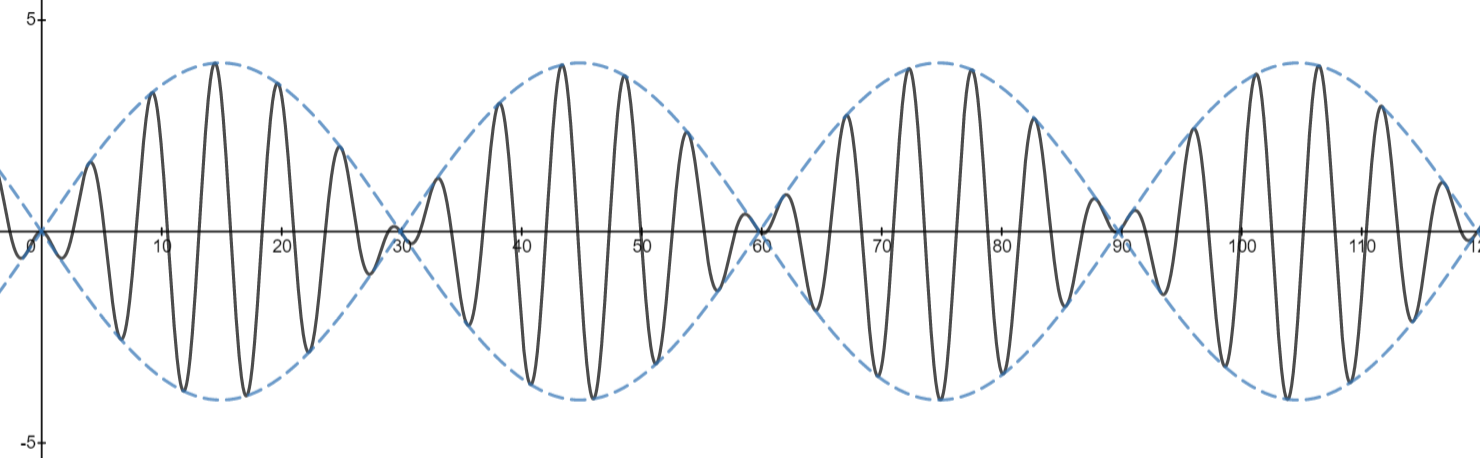
\includegraphics[width=0.75\textwidth]{./higherOrder/forcedVibrs/beats.png}
\end{center}
\subsubsection{Resonance ($\omega = \gamma$)}
\noindent
In the case where $\omega = \gamma$, we need to add an extra factor of $t$ to our guess for $y_p$. So,
\begin{equation*}
	y_p = At\cos{(\omega t)} + Bt\sin{(\omega t)}
\end{equation*}
Solving for $A$ and $B$,
\begin{equation*}
	my_p'' + ky_p = 2Bm\omega\cos{(\omega t)} - 2Am\omega\sin{(\omega t)} = F_0\cos{(\omega t)}
\end{equation*}
\begin{equation*}
	\implies A = 0 \text{ and } B = \frac{F_0}{2m\omega}
\end{equation*}
So our solution is,
\begin{equation*}
	y = C_1\cos{(\omega t)} + C_2\sin{(\omega t)} + \frac{F_0}{2m\omega}t\sin{(\omega t)}
\end{equation*}\\

\noindent
Let's look specifically at the IVP where $y(0) = 0$ and $y'(0) = 0$.
\begin{equation*}
	C_1 = C_2 = 0
\end{equation*}
So,
\begin{equation*}
	y = \frac{F_0}{2m\omega}t\sin{(\omega t)}
\end{equation*}\\

\noindent
Here, the amplitude grows with $t$, creating bigger and bigger waves. This is resonance, and you can see mathematically how it is responsible for one string causing another tuned the same to vibrate and the collapsing of bridges.

\begin{center}
	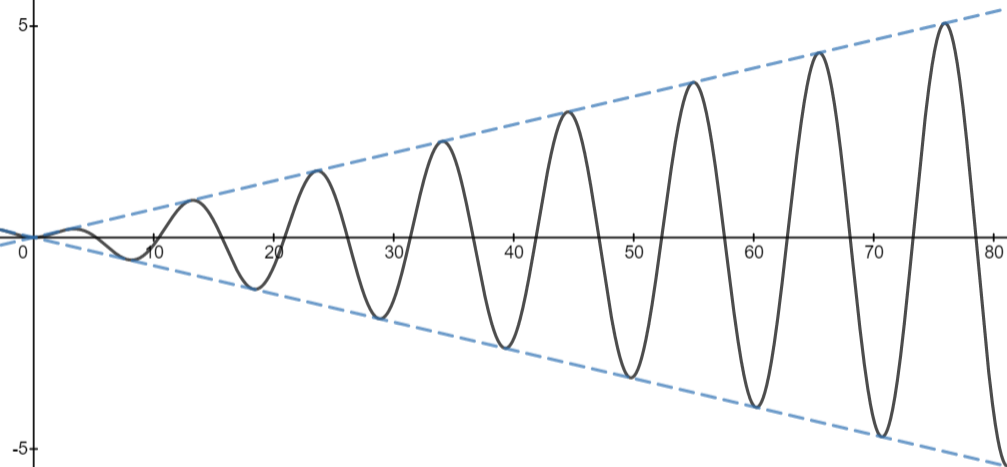
\includegraphics[width=0.75\textwidth]{./higherOrder/forcedVibrs/resonance.png}
\end{center}